\documentclass{sig-alternate}
\usepackage{graphicx}
\usepackage{eepic}

\begin{document}

\conferenceinfo{DEBS}{2009 Nashville, Tennessee USA}

\title{Passing Actor Continuations}
\subtitle{Efficient and Extensible Request Handling for Event-Driven Architectures}

\numberofauthors{1} 

\author{
\alignauthor
Stefan Plantikow\\
       \affaddr{Zuse Institute Berlin (ZIB)}\\
       \affaddr{Takustrasse 7}\\
       \affaddr{14195 Berlin, Germany}\\
       \email{plantikow@zib.de}
}

\date{16 May 2009}


\maketitle

\begin{abstract}

The logic for handling of application requests to an event-driven architecture is often distributed
over different portions of the source code. This complicates changing and understanding the flow
of events in the system.

The article presents an approach that allows extracts request handling logic from regular stage
functionality into a a set of request scripts. Application requests are executed step-wise according
to their script by sending continuations that encapsulate their request's current execution state to
stages for local processing and optional forwarding of follow-up continuations. The implementation
of a domain specific language for request scripts for the scala actor library is described that aims
to simplify writing of request handling code. Evaluation results indicates that request handling
with actor continuations performs about equally or better to using separate stages for request
routing logic for scripts of at least 3 sequential steps.

\end{abstract}

\category{H.2.4}{Information Systems}{Systems}[Concurrency]         
\category{D.1.3}{Software}{Programming Techniques}[Concurrent Programming]         
\category{D.3.3}{Programming Languages}{Language Constructs and Features}[Concurrency]
%\category{D.2.11}{Software Engineering}{Distribution, Maintenance, and Enhancement}[Extensibility]

\keywords{Request Routing, Event-Driven Architecture, Partial Continuation, Actor Model, Scala}


\section{Introduction}             

Staged, event-driven architectures~\cite{Welsh:2009} implement an approach to the design of
server software that can provide high degrees of concurrency and throughput. This is achieved by
structuring the software as a set of stages. Stages run in separate threads, do not share state, and
communicate exclusively via event queues, i.e. follow the actor model of message passing
concurrency.

Requests to the server application are enqueued as events at some stage. Processing such an event
may involve pure local computation, accessing stage-specific functionality (like manipulating state
and resources), and continuing request handling by sending new events to other stages.

The resulting interactions during request handling at runtime can be complex and difficult to
understand. Thererfore, to help understandability, all logic for handling a certain type of request
should at least be implemented in a readable, singular section of the source code. However, when a
new application request type is added to a staged architecture, the processing logic is typically
spread over the implementations of all involved stages and often requires the introduction of new
event types.

Staged architectures suffer from distribution of application request handling logic over different
stages. This reduces the understandability of the system and makes it harder to modify the handling
of application requests. Additionally, it impedes the addition of new request types without changing
the source code of existing stages and redeploying large parts of the system.

In this article, an approach for extracting the implementation of application request handling logic
into separate source code units that are independent of the implementation of core stage
functionality is presented. The solution is based on sending partial continuations between stages
and CPS-transformation of request handling code. It is unique in that it does neither require
additional messages nor leads to source code with deeply nested callbacks. The approach has been
implemented as a domain specific languages~(DSL) for the scala actors library~\cite{Haller:2007}.


\section{Separating request and stage}

The distribution of request handling logic over the system stems from the intertwining of code for
pure local computation and code that actually has to be performed at a specific stage. For a given
request, pure computational code is glued together with one of its surrounding blocks of
stage-specific code quite randomly. Required intermediary values are sent as part of the event
that triggers a block's execution.

% This cuts down the design space unneccesarily. To implement application request handling, an
% architecture needs (1) a way to execute stage-specific code at its stage (2) a mechanism for
% executing non-stage specific code at some stage (3) a way to transfer intermediary values between
% stages, and (4) preserve the execution order between different kinds of code blocks
% (synchronization).

Extracting request logic requires a mechanism for pausable, stateful control-flow. One approach to
this is the use of additional coordination stages. A request's non stage-specific code is executed
by a coordinator stage. Stage-specific functionality is executed by sending and receiving events.
This solution has drawbacks: Executing stage-specific code requires the sending of two messages,
requires a context switch back to the coordinator stage (e.g. to access pre-request state) and the
introduction of matching event types. Additionally, special care is necessary to avoid overloading
of coordinator stages by implementing them in a non-blocking fashion and by load-balancing over
them.

The \emph{continuation} of a computation at a point in time describes the part of a computation that
yet needs to be computed. A continuation may be explicitly stored as a value by reifying it as an
anonymous function. It may then be executed arbitrary often by calling this function.

This may be used to implement pausable, stateful control-flow: Stages receive events that actually
are anonymous functions that represent the current continuation of some request. Such incoming
continuations are executed by calling them with the executing stage as their sole argument. Through
this means request continuations gain access to the functionality of local stages. When the
execution of a request continuation at a stage is about to finish, the follow-up continuation may be
captured in a last step. This follow-up continuation is then simply sent to the next stage where
request handling continues.

This \emph{actor continuation passing (ACP)} approach does not require any intermediate stages for
the execution of the request handling logic and thus avoids the introduction of additional messages.
It does not require special events for communicating intermediary values since continuations contain
their stack frame at capture time. On the downside, it requires some overhead for continuation
capturing. The impact of these different properties will be shown in the evaluation section.


\section{A Request Handling DSL}

Souffleuse is a library for request handling with actor continuation passing that has been
implemented in the scala programming language~\cite{Odersky:2004} using the scala actor
library~\cite{Haller:2007}. Sofleuse provides a \emph{domain specific language (DSL)} for writing
request scripts that execute over a set of locally running stages. Request scripts are implemented
in terms of a simple set of commands that allow structuring scripts as a sequence of code blocks
that are executed at different stages.

The command set includes: \textbf{remember(\emph{value})} for remembering intermediary values,
\textbf{compute(\emph{code-thunk})} for computing at the current local stage, \textbf{goto(\emph{stage})}
for changing the locus of computation to another stage, and \textbf{yield(result)} for delivering a
result. Scripts are either run blocking or non-blocking. As an example, consider the implementation
of a single remote procedure call:
                    
\medskip   
{\footnotesize\begin{tabular}{l}           
$\textbf{def}\ $rpc$(\emph{targetStage}, \emph{args})\ =\ \{$\\	
\hspace{2ex} $\textbf{val}\ \emph{request}\ =\ \textbf{for} ($\\
\hspace{6ex} $\emph{stageRep}\ \leftarrow\ $goto$(\emph{targetStage})$\\
\hspace{6ex} $\emph{procResult}\ \leftarrow\ $compute$\ \{\ stageRep.$proc$(\emph{args})\ \}$\\
\hspace{2ex} $)\ \textbf{yield}\ procResult$\\
\hspace{2ex} $\textbf{return}\ $run$(\emph{request})$\\   
$\}$\\
\end{tabular}}
\medskip

The call is wrapped as a function that initially assembles a new request script. The script itself first
transfers the execution to the \emph{targetStage} for the RPC using \textbf{goto}. Then, the actual
RPC is executed at that stage using \textbf{compute}, and finally the return value is yielded. To
actually execute this request script, it is started with \textbf{run}.




% \begin{figure*}[t]
% \begin{center}
% 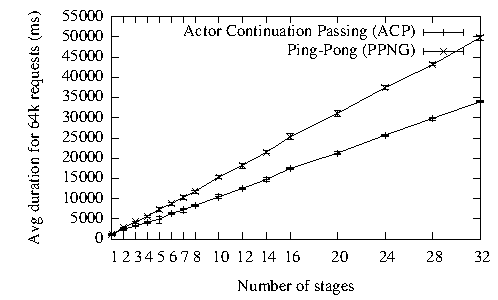
\includegraphics[width=.33\hsize]{plots/BENCHMARK-8CORE-2009-03-01-23:59-LIN.pdf}%
% 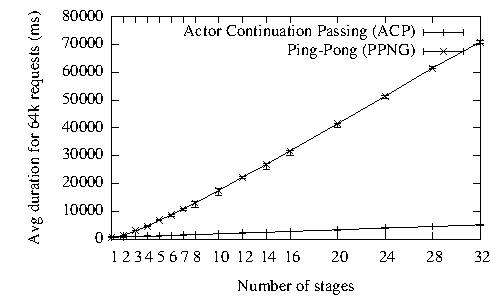
\includegraphics[width=.33\hsize]{plots/BENCHMARK-8CORE-2009-03-01-23:59-BLK.pdf}%
% 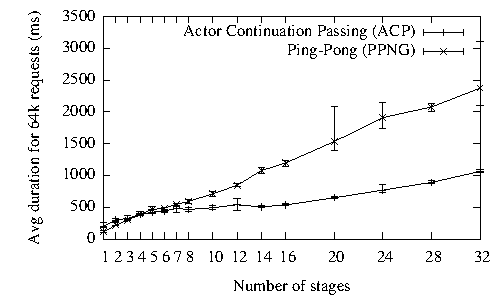
\includegraphics[width=.33\hsize]{plots/BENCHMARK-8CORE-2009-03-01-23:59-ALL.pdf}
% \end{center}
% \end{figure*}
	

\section{Implementation Details}

Stages are implemented as actors that run in separate threads (receive-actors in scala parlance).
Their main loop listens for messages consisting of one-argument anonymous lambda-functions. When
such a function is received, it is executed and given access to the stage by passing the stage as
its first argument. This is sufficient to implement request handling by explicitely writing out
continuation functions in the source code and by sending them to the stages via normal message
passing. However, this can lead to unreadable source code with a nesting level of anonymous lambda
functions that is as large as the number of sequentially passed stages.

Instead, Souffleuse implements request routing with actor continuation passing through CPS-transform
and message sending at stage boundaries. \emph{Continuation Passing Style (CPS)} is a control flow
graph transformation that replaces regular function return with calling a continuation function that
is passed as an extra argument.

In Souffleuse, to capture continuations, commands are chained by using scala's
CPS-transforming-\textbf{for}-generator-expressions. For example, \textbf{goto} converts the given
stage into a generator that sends the continuation lambda for the remainder of the for-expression to
the stage via message sending where it is executed as described above.

% Souffleuse does not support exception handling across stage boundaries, does not perform
% tail-call-optimization, and has no native syntax support for non-sequential control-flows.


\section{Evaluation}

Souffleuse has been compared against using coordinator stages in a
messages-around-a-ring-of-stages-scenario with different load generation strategies. The results
indicate that it performs equally or better when the ring size is $\ge$~3. With rising ring size,
Soufflese converges towards a twofold performance increase since the required number of messages is
halved. The use of complex events consisting of continuation functions appears to have neglible
overhead. All tests were conducted on a 8-core machine.


\section{Summary}                                          

The results indicate that actor continuation passing is a viable approach for separating request
handling from stage functionality without suffering from the performance penalty introduced by using
explicit coordinator stages. Souffleuse implements this approach as a mini-DSL in scala. The
implementation eliminates the need for deeply nested callbacks by using the implicit
CPS-transformation of scala's \textbf{for}-expression. Thus writing application request handling
logic as fast and concise request scripts is enabled.

\section{Acknowledgments}

The author thanks Bj\"orn Kolbeck who initially described the problem in the context of XtreemFS,
a distributed filesystem implemented as a staged architecture.
           
\bibliographystyle{abbrv}
\bibliography{sigproc}  

\end{document}
